%------------------------------------------
%	$Id: GMT_Appendix_C.tex,v 1.15 2007-03-20 23:26:34 remko Exp $
%
%	The GMT Documentation Project
%	Copyright 2000-2007.
%	Paul Wessel and Walter H. F. Smith
%------------------------------------------
%

\chapter{Including \gmt\ graphics into your documents}
\thispagestyle{headings}
\label{app:C}
\index{GMT@\GMT!graphics in documents}
\index{documents!include GMT@\GMT graphics}

Now that you made some nice graphics with \GMT, it is time to add them to a document, an article, a report, your dissertation, a poster, a web page, or a presentation. Of course, you could try the old-fashioned scissors and glue stick. More likely, you want to incorporate your graphics electronically into the document. Depending on the application, the \GMT\ \PS\ file will need to be converted to Encapsulated \PS\ (EPS), PDF, or some raster format in order to incorporate them into the document.
\begin{itemize}
\item When creating a document intended for printing (article, dissertation, or poster) it is best to preserve the scalable vector characteristics of the \PS\ file. Many applications can directly incorporate \PS\ in the form of EPS files. Modern programs will often allow the inclusion of PDF files. Either way, the sharpness of lines and fonts will be preserved and can be scaled up or down as required.
\item When the aim is to display the graphics on a computer screen or project it using a computer projector, it is wise to convert the \PS\ into a raster format (e.g., JPG, PNG, TIFF). Although applications like \progname{PowerPoint} can do this for you, you can best take the conversion into your own hands for the best results.
\end{itemize} 
This Chapter will give some examples of incorporation of \GMT\ graphics into documents and how to achieve the best quality results.

\section{Making \gmt\ Encapsulated \PS\ and PDF Files}
\index{PostScript@\PS!encapsulated (EPS)}
\index{PostScript@\PS!convert to PDF}
\index{PostScript@\PS!BoundingBox}
\index{EPS file}
\index{PDF file}

\GMT\ can produce both freeform \PS\ files and the more
restricted Encapsulated \PS\ files (EPS).  The former is
intended to be sent to a printer or \PS\ previewer, while
the latter is indended to be included in another document
(but should also be able to print and preview).  You
control what kind of \PS\ that \GMT\ produces by manipulating
the {\bf PAPER\_MEDIA} parameter (see the \GMTprog{gmtdefaults} man
page for how this is accomplished).  Note that a freeform \PS\
file may contain special operators (such as \texttt{Setpagedevice})
that is specific to printers (e.g., selection of paper tray).
Some previewers (among them, Sun's \progname{pageview}) do not
understand these valid instructions and may fail to image the file. Also, embedding freeform \PS\ with such instructions in it into a larger document can create printing to fail.
While you could choose another viewer (we recommend \progname{ghostview}) to view single plots prepared by \GMT, it is generally wiser to select EPS output when you are creating a plot intended for inclusion into a larger document. Some programs (and some publishers as well) do not allow the use of instructions like \texttt{Setpagedevice} as part of embedded graphics.

An EPS file that is to be placed into another document
needs to have correct bounding box
parameters.  These are found in the \PS\ Document
Comment \%\%BoundingBox.  Applications that generate EPS
files should set these parameters correctly.  Because \GMT\
makes the \PS\ files on the fly, often with several
overlays, it is not possible to do so accurately.  However,
\GMT\ does make an effort to ensure that the BoundingBox is
large enough to contain the entire composite plot\footnote{In contrast,
regular \GMT\ \PS\ files simply have
a \%\%BoundingBox that equal the size of the chosen paper.}.
Therefore, if you need a ``tight'' BoundingBox you need to post-process
your \PS\ file.  There are several ways in which this
can be accomplished.

\begin{itemize}
\item Programs such as Adobe \progname{Illustrator}, Aldus
\progname{Freehand}, and Corel \progname{Draw} will allow you
to edit the boundingbox graphically.

\item A command-line alternative is to use freely-available program \progname{epstool} from the makers of Aladdin \progname{ghostscript}.  Running
\small
\begin{verbatim}
epstool -c -b myplot.ps
\end{verbatim}
\normalsize
should give a tight BoundingBox; \progname{epstool} assumes the plot
is page size and not a huge poster.

\item Another option is to use \progname{ps2epsi} which also comes with the \progname{ghostscript} package.  Running
\small
\begin{verbatim}
ps2epsi myplot.ps myplot.eps
\end{verbatim}
\normalsize
should also do the trick. The downside is that this program adds an "image" of the plot in the preamble of the EPS file, thus increasing the file size significantly. On the other hand, some programs rely on the presence of this image to show the plot while editing your document.

\item If you also intend to convert the document into PDF or raster image, we suggest you use the \GMT\ supplementary program \GMTprog{ps2raster} instead. The \Opt{A} option will first figure out the tight BoundingBox. For example, running
\small
\begin{verbatim}
ps2raster -A -Tf myplot.ps
\end{verbatim}
\normalsize
will convert the \PS\ file \filename{myplot.ps} into a PDF file \filename{myplot.pdf} which is exactly cropped to the tightest possible BoundingBox.
\end{itemize}

If you do not want to modify your illustration but just include it in a text document: many word processors (such
as Microsoft \progname{Word}, Corel \progname{WordPerfect}, and Apple \progname{Pages})
will let you include a \PS\ file that you may place but not edit. Newer versions of those programs also allow you to include PDF versions of your graphics. Except for \progname{Pages}, 
you will not be able to view the figure on-screen, but it will print correctly.

\section{Example: Including \gmt\ graphics into \LaTeX}
\index{LaTeX@\LaTeX}

All illustrations in this \GMT\ documentation were \GMT-produced \PS\ files. They were converted to PDF files using \GMTprog{ps2raster} and then included into a \LaTeX\ document that was processed with \progname{pdflatex} to create the PDF document you are reading.

Conversion from \PS\ to PDF can best be performed with the \GMT\ supplementary program \GMTprog{ps2raster}. It is designed to provide the best quality PDF files using \progname{ghostscript} as a rendering engine. The program \GMTprog{ps2raster} avoids anti-aliasing and lossy compression techniques that are default to \progname{ghostscript} and includes the fonts into the resulting PDF file to ensure portability. By default the fonts are rendered at 720 dots-per-inch, but that can be changed with the \Opt{E} option. Simply run
\small
\begin{verbatim}
ps2raster -A -Tf *.ps
\end{verbatim}
\normalsize
to convert all \PS\ files to PDF while cropping it to the smallest possible BoundingBox.

Next, add the graphics into the \LaTeX\ document using the \verb|\includegraphics| command supplied by the \textsf{graphicx} package. In the preamble of your \LaTeX\ document you will need to include the line
\small
\begin{verbatim}
\usepackage{graphicx}
\end{verbatim}
\normalsize
The inclusion of the graphics will probably be inside a floating figure environment; something like this
\small
\begin{verbatim}
\begin{figure}
   \includegraphics{myplot}
   \caption{This is my first plot in \LaTeX.}
   \label{fig:myplot}
\end{figure}
\end{verbatim}
\normalsize
Note that the \verb|\includegraphics| command does not require you to add the suffix \verb|.pdf| to the file name. If you run \progname{pdflatex}, it will look automatically for \filename{myplot.pdf}. If you run \progname{latex}, it will use \filename{myplot.eps} instead.

You can scale your plot using the options \verb|width=| or \verb|height=|. In addition, if your original graphics was produced in landscape mode (i.e., you did not use \GMT's \Opt{P} option), you will need to rotate the plot as well. For example,
\small
\begin{verbatim}
\includegraphics[angle=-90,width=0.8\textwidth]{myplot}
\end{verbatim}
\normalsize
will rotate the image 90\DS\ clockwise and scale it such that its width will be 80\% of the width of the text column.

\section{Converting \gmt\ graphics to raster image}
\index{PostScript@\PS!convert to raster image}
\index{PNG file}

For some applications it is practical or even essential that you \PS\ file is converted into a raster format, such as GIF (Graphics Interchange Format), TIFF (Tagged Image File Format), PNG (Portable Network Graphics), or JPEG (Joint Photographic Experts Group). A web page is better served with a raster image that will immediately show on a web browser, than a \PS\ file that needs to be downloaded to view, despite the better printing quality of the \PS\ image. A less obvious reason to convert your image to a raster format is to by-pass \progname{PowerPoint}'s rendering engine in case you want to embed the image into a presentation.

Of all the image formats we strongly recommend to use the PNG format because it can be made non-lossy, has good compression, and allows a basically unlimited number of colors. Again, there are a view options to perform the conversion from \PS\ to PNG.
\begin{itemize}
\item The \progname{ImageMagick} package comes with a command-line tool \progname{convert} which using \progname{ghostscript} as a rendering engine. Although its basic syntax is quite easy:
\small
\begin{verbatim}
convert myplot.ps myplot.png
\end{verbatim}
\normalsize
it requires some knowledge of image processing to supply all the right options to get it to produce a high quality image with the right resolution. For example, the default anti-aliasing option should be switched off as we will show below. 

\item The \GMT\ supplemental program \GMTprog{ps2raster} can do the conversion for you much more efficiently. Simply type
\small
\begin{verbatim}
ps2raster -A -Tg *.ps
\end{verbatim}
\normalsize
to convert all \PS\ files to PNG while cropping it to the smallest possible BoundingBox. The default image resolution is 300 dpi, but can be adjusted using the \Opt{E} option.
\end{itemize}

\section{Example: Including \gmt\ graphics into \progname{PowerPoint}}

\begin{figure}
   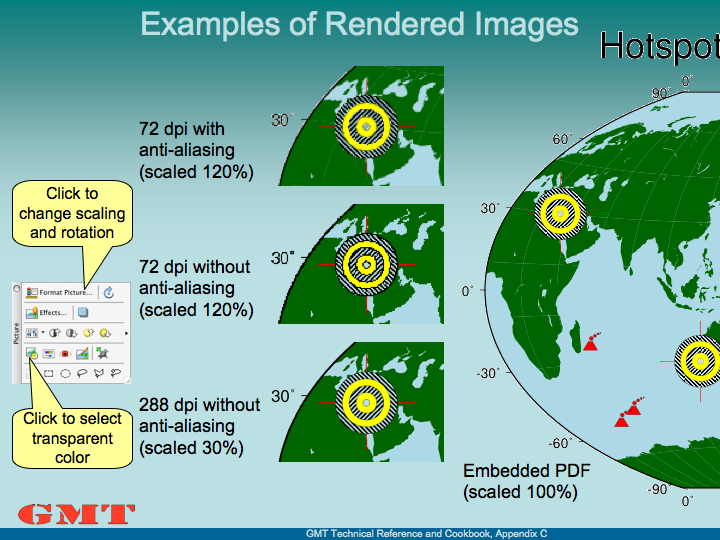
\includegraphics[width=\textwidth,bb=0 0 720 540]{ppt/rendering.png}
   \caption{Examples of rendered images in a \protect\progname{PowerPoint} presentation.}
   \label{fig:rendering}
\end{figure}

In Figure~\ref{fig:rendering} we have attempted to include the result of example 20 into a \progname{PowerPoint} presentation. First the \PS\ file was converted to PDF (using \GMTprog{ps2raster}), then loaded into \progname{PowerPoint} and the white color was made transparent using the formatting toolbar. Clearly, when we let \progname{PowerPoint} do the rendering, we do not get the best result:\begin{enumerate}
\item The anti-aliasing causes the tiles that make up the land to stand out. This is because the anti-aliasing algorithm blurs all edges, even when the tiles join seamlessly.
\item The background color was assumed to be white, hence the text is "smoothed" using gray shades, instead shades of blue which would be appropriate for the background we are using.
\end{enumerate}

On the left of Figure~\ref{fig:rendering} we have included PNG versions of a portion of the same example. This shows the workings of anti-aliasing and different resolutions. Just switching anti-aliasing off is clearly not an option either. It is true that we got rid of the gray blurring and the seams between the tiles, but without anti-aliasing the image becomes very blocky. The solution is to render the image at a higher resolution (e.g., 300 dpi) and then shrink the image to the appropriate size. The scaling, rotation as well as the selection of the transparent color can be accomplished with the formatting toolbar of \progname{PowerPoint}, which can be found by selecting and right-clicking the included image.

\section{Concluding remarks}

These examples do not constitute endorsements of the products mentioned above; they only represent our limited experience with adding \PS\ to various types of documents.  For other solutions and further help, please post messages to
\htmladdnormallink{gmt-help@hawaii.edu}{mailto:gmt-help@hawaii.edu}.
